\documentclass[11pt,a4paper]{article}

\usepackage[T1]{fontenc}
\usepackage[utf8]{inputenc}
\usepackage{lmodern}
\usepackage{geometry}
\usepackage{graphicx}
\usepackage{booktabs}
\usepackage{array}
\usepackage{amsmath}
\usepackage{amssymb}
\usepackage{siunitx}
\usepackage{xcolor}
\usepackage{hyperref}
\usepackage{caption}
\usepackage{subcaption}

\geometry{margin=2.1cm}
\graphicspath{{figures/}}
\hypersetup{
  colorlinks=true,
  linkcolor=blue!55!black,
  citecolor=blue!55!black,
  urlcolor=blue!55!black
}

\sisetup{
  detect-all=true,
  group-separator={,},
  group-minimum-digits=4
}

\newcommand{\RMSE}{\mathrm{RMSE}}
\newcommand{\MAE}{\mathrm{MAE}}
\newcommand{\ms}{m_s}
\newcommand{\Czon}{C_{\mathrm{zon}}}
\newcommand{\Tzone}{T_{\mathrm{zone}}}
\newcommand{\Tsupply}{T_{\mathrm{sup}}}
\newcommand{\That}{\widehat{T}}
\newcommand{\Phat}{\widehat{P}}

\title{Results I: Digital Twin Fidelity and RL-Utility Gap}
\author{Standalone Overleaf-ready Block 1 section}
\date{}

\begin{document}
\maketitle

\begin{abstract}
This standalone section expands the Results I block of the Q1 manuscript. It
documents the control-oriented v3 surrogate, the physically informed v3.5
surrogate, the three-stage Stage A/B/C inverse calibration protocol, the
matched-corpus control experiment, runtime feasibility, the hybrid backend, and
the fidelity-to-RL gap. The main conclusion is deliberately asymmetric:
calibrated v3.5 is supported as a predictive digital twin, but rejected as a
direct reinforcement-learning rollout backend. The constructive solution is a
hybrid role assignment: v3 supplies smooth rollout dynamics, while frozen v3.5
contributes a physical disagreement penalty.
\end{abstract}

\tableofcontents
\newpage

\section{Block 1 objective and evidence boundary}

Block 1 establishes the empirical foundation for the central scientific claim
of the project: predictive fidelity and reinforcement-learning training utility
are different objectives. A surrogate can be excellent as a digital twin and
still fail as a direct policy-training environment.

The block evaluates two surrogate families for the BOPTEST
\texttt{bestest\_air} testcase:
\begin{itemize}
  \item \textbf{v3}: a compact control-oriented black-box surrogate designed
  for smooth PPO rollouts.
  \item \textbf{v3.5}: a physically informed RC-NeuralODE-style surrogate with
  an identifiable zone thermal capacitance \(\Czon\), calibrated through Stage
  A/B/C inverse identification.
\end{itemize}

\begin{figure}[htbp]
  \centering
  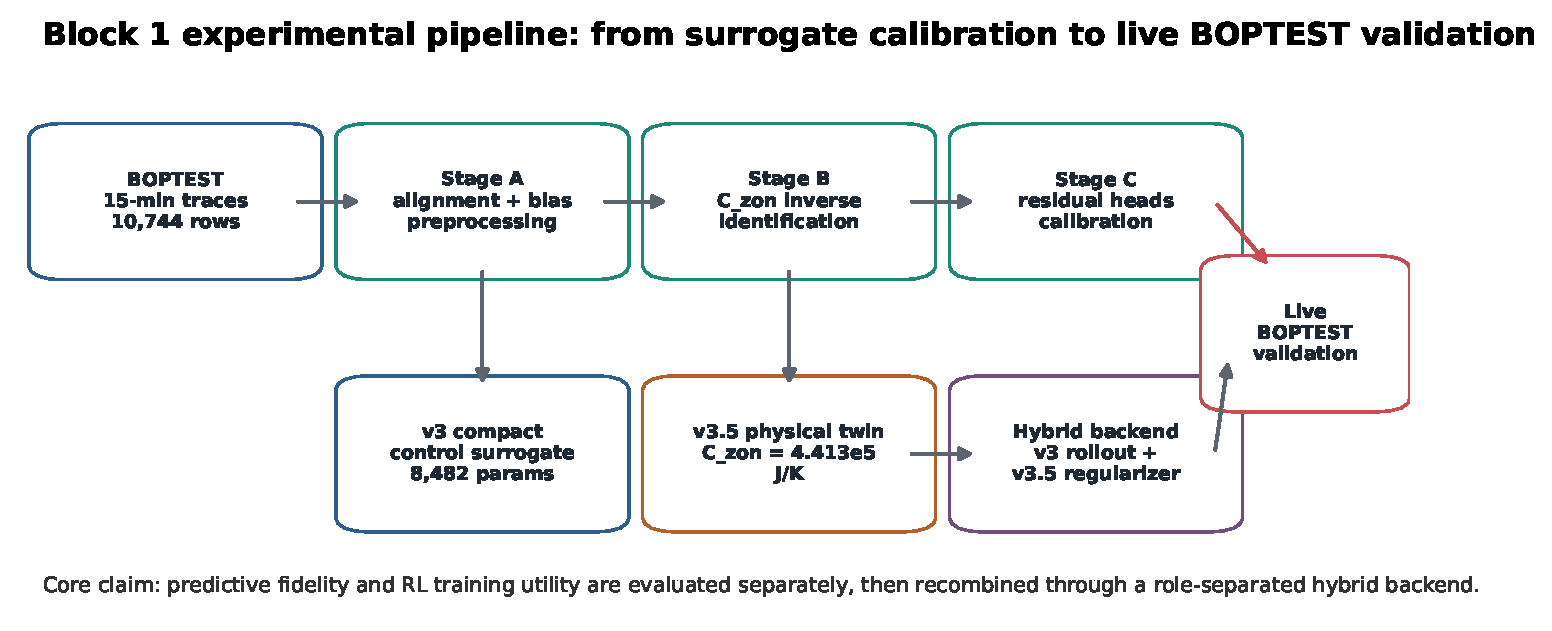
\includegraphics[width=0.95\linewidth]{block1_q1_fig01_pipeline.pdf}
  \caption{Block 1 experimental pipeline: BOPTEST telemetry, v3/v3.5 surrogate
  construction, Stage A/B/C calibration, offline validation, live BOPTEST
  controller validation, and hybrid backend construction.}
  \label{fig:pipeline}
\end{figure}

The evidence boundary is important. Block 1 does not claim that calibrated v3.5
is the best controller backend. It first validates v3.5 as a predictive digital
twin, then shows that this stronger predictive fidelity does not translate into
direct RL utility. The hybrid backend is introduced only after this negative
result is established.

\section{Control-oriented surrogate v3}

\subsection{Data collection and modeling role}

The v3 surrogate is the workhorse model used for PPO rollout generation. The
canonical historical v3 checkpoint was trained on a \(51\,200\)-row hourly
closed-loop BOPTEST corpus. For reviewer mitigation, a matched v3 branch was
also trained on the same \(10\,744\)-row, \(\SI{900}{s}\) corpus used by v3.5.
This matched branch is used only for attribution of predictive-fidelity gains;
the downstream Block 2 and Block 3 controller experiments retain the original
canonical v3 rollout backend.

The v3 feature vector is deterministic and bounded. It contains normalized zone
temperature, normalized ambient temperature, cyclic time encodings, cyclic
season encodings, and the previous two action components. In compact form,
\begin{equation}
  x_t =
  \left[
    T_{\mathrm{zone,norm}},
    T_{\mathrm{amb,norm}},
    \sin(2\pi h/24),
    \cos(2\pi h/24),
    \sin(2\pi d/365),
    \cos(2\pi d/365),
    a_{0,t-1},
    a_{1,t-1}
  \right].
  \label{eq:v3-input}
\end{equation}

\begin{table}[htbp]
\centering
\caption{v3 input feature vector.}
\label{tab:v3-input}
\begin{tabular}{clll}
\toprule
Index & Feature & Normalization & Physical meaning \\
\midrule
0 & \(T_{\mathrm{zone,norm}}\) & affine \(15..35^\circ C\rightarrow[-1,+1]\) & current zone temperature \\
1 & \(T_{\mathrm{amb,norm}}\) & affine \(-10..40^\circ C\rightarrow[-1,+1]\) & outdoor temperature \\
2 & \(h_{\sin}\) & \(\sin(2\pi h/24)\) & daily phase \\
3 & \(h_{\cos}\) & \(\cos(2\pi h/24)\) & daily phase \\
4 & \(d_{\sin}\) & \(\sin(2\pi d/365)\) & seasonal phase \\
5 & \(d_{\cos}\) & \(\cos(2\pi d/365)\) & seasonal phase \\
6 & \(a_0\) & normalized supply command & previous supply-temperature command \\
7 & \(a_1\) & normalized fan/intensity command & previous fan command \\
\bottomrule
\end{tabular}
\end{table}

\subsection{v3 architecture and hyperparameters}

The v3 model is not a generic MLP. It is a dual-head surrogate:
\begin{align}
  \Delta \widehat{T}_{t+1} &= f_{\theta,T}(x_t), \\
  \widehat{P}_{t+1} &= f_{\theta,P}(x_t).
\end{align}
The next temperature prediction is
\begin{equation}
  \widehat{T}_{t+1}=T_t+\Delta \widehat{T}_{t+1}.
  \label{eq:v3-temperature-update}
\end{equation}

\begin{figure}[htbp]
  \centering
  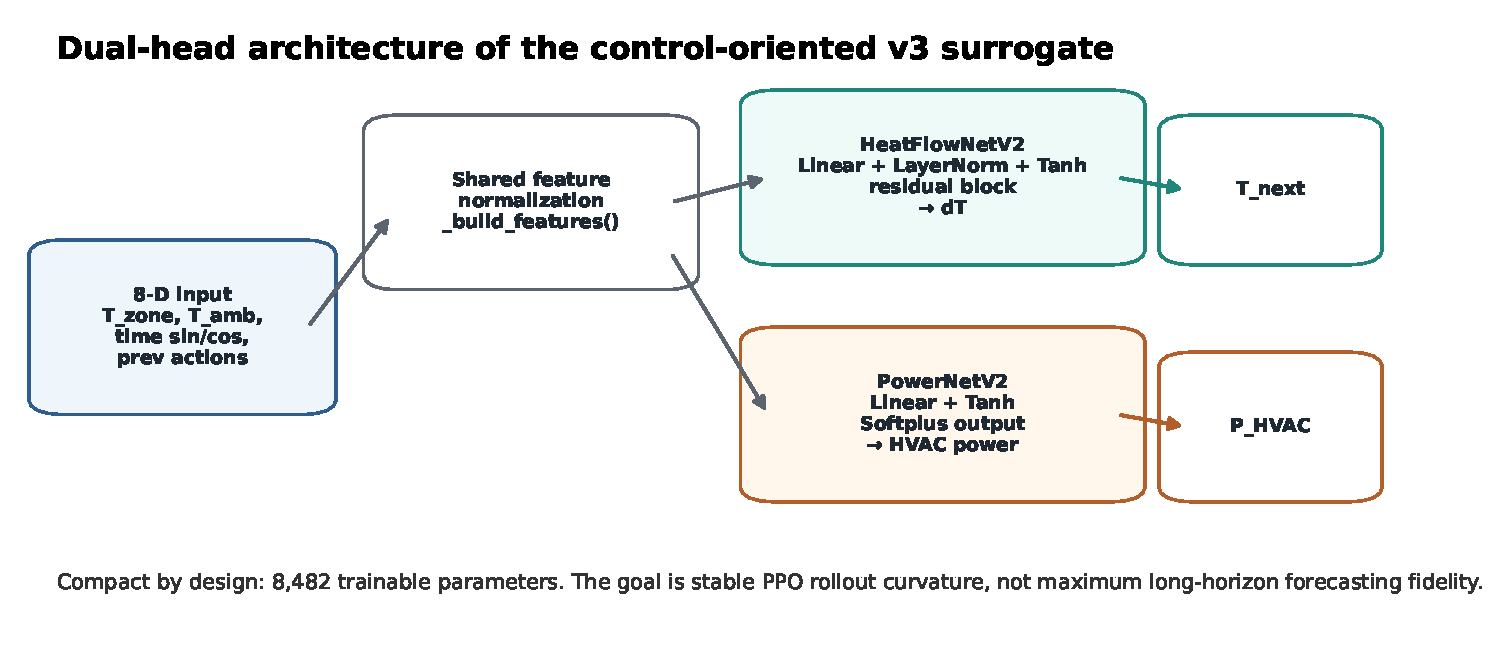
\includegraphics[width=0.95\linewidth]{block1_q1_fig02_v3_dual_head.pdf}
  \caption{v3 dual-head architecture. The HeatFlowNetV2 head predicts
  \(\Delta T\), the PowerNetV2 head predicts HVAC power, and the full model has
  \(8\,482\) trainable parameters.}
  \label{fig:v3-architecture}
\end{figure}

\begin{table}[htbp]
\centering
\caption{v3 architecture and training configuration.}
\label{tab:v3-hyperparams}
\begin{tabular}{p{0.27\linewidth}p{0.66\linewidth}}
\toprule
Property & Value \\
\midrule
Temperature head & Linear(8--64)+LayerNorm+Tanh \(\rightarrow\) Linear(64--64)+LayerNorm+Tanh with residual connection \(\rightarrow\) Linear(64--32)+Tanh \(\rightarrow\) Linear(32--1) \\
Power head & Linear(8--32)+Tanh \(\rightarrow\) Linear(32--32)+Tanh \(\rightarrow\) Linear(32--1)+Softplus \\
Activation design & Tanh + LayerNorm + residual connection \\
Trainable parameters & \(8\,482\) total: \(7\,105\) temperature head, \(1\,377\) power head \\
Optimizer & AdamW, learning rate \(10^{-3}\), weight decay \(10^{-4}\) \\
Scheduler & CosineAnnealingLR \\
Batch size & 256 \\
Early stopping & patience 30, improvement threshold \(10^{-6}\) \\
Canonical training result & best epoch 184 / 215, one-step validation RMSE \(\SI{0.6255}{\celsius}\), \(R^2=0.9794\) \\
\bottomrule
\end{tabular}
\end{table}

The Tanh+LayerNorm design is deliberately smooth. For RL rollout generation,
the surrogate must provide stable local action-response surfaces; this is a
different requirement from long-horizon predictive accuracy.

\section{Physically informed surrogate v3.5}

\subsection{Why v3.5 is needed}

The v3.5 surrogate introduces a physical backbone. Its central physical
parameter is the zone thermal capacitance \(\Czon\). The motivation is
interpretability and transfer: \(\Czon\) is a building property rather than a
policy artifact.

The v3.5 workflow is split into three stages:
\begin{description}
  \item[Stage A] telemetry preprocessing and alignment;
  \item[Stage B] inverse identification of \(\Czon\);
  \item[Stage C] residual-head refinement with \(\Czon\) frozen.
\end{description}

\subsection{Stage A: telemetry alignment}

Stage A removes effects that should not be misidentified as building physics:
latency, constant temperature bias, and global power-channel scaling. The
canonical Stage A result uses a 1-step latency compensation, corresponding to
\(\SI{15}{min}\), and a temperature bias correction of approximately
\(-\SI{0.1049}{\celsius}\). The post-alignment temperature RMSE is about
\(\SI{0.2383}{\celsius}\).

\subsection{Stage B: inverse identification of \(\Czon\)}

Stage B solves a one-parameter inverse problem for the physical capacitance. To
avoid letting quasi-steady samples dominate the inverse problem, the calibration
uses only the high-excitation subset: 403 of 8058 training rows, corresponding
to the top excitation quantile.

The prior and final estimates are
\begin{align}
  \Czon^{\mathrm{prior}} &= 4.200\times10^5~\mathrm{J/K},\\
  \Czon^{\mathrm{final}} &= 4.413\times10^5~\mathrm{J/K}.
\end{align}
The relative update is
\begin{equation}
  \eta_C
  =
  \frac{\Czon^{\mathrm{final}}-\Czon^{\mathrm{prior}}}
       {\Czon^{\mathrm{prior}}}
  =
  \frac{4.413-4.200}{4.200}
  \approx 0.0507
  =
  5.1\%.
  \label{eq:czon-update}
\end{equation}
This is the desired magnitude: large enough to show data-driven identification,
small enough to remain physically plausible.

\begin{figure}[htbp]
  \centering
  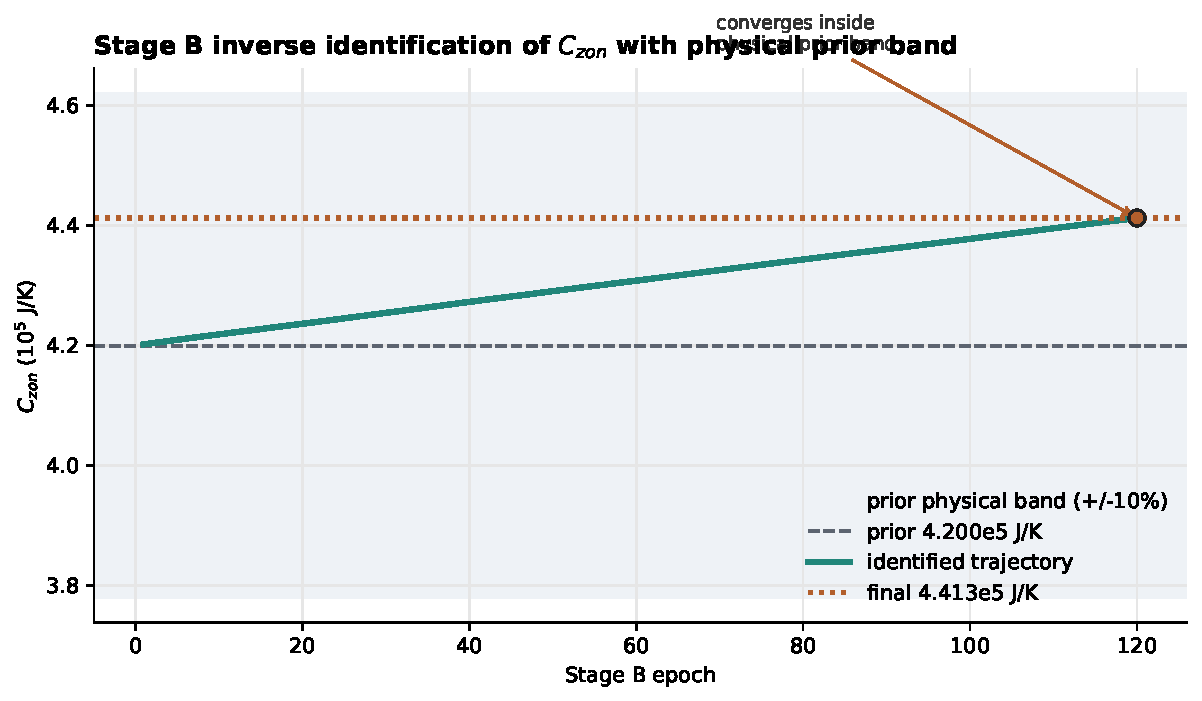
\includegraphics[width=0.95\linewidth]{block1_q1_polish_czon_prior_band.pdf}
  \caption{Stage B \(\Czon\) identification with a physical prior band. The
  shaded region denotes the \(\pm 10\%\) prior plausibility interval around
  \(4.200\times10^5\) J/K; the identified value converges inside this physical
  band rather than escaping as an unconstrained neural parameter.}
  \label{fig:stage-abc}
\end{figure}

\subsection{Stage C: residual-head refinement}

Stage C refines residual neural heads on top of the frozen physical backbone.
The canonical implementation is two-step: first, an episode-aware run calibrates
temperature and rollout behavior; second, a power-head-only run improves the
power channel while preserving the identified \(\Czon\).

\begin{table}[htbp]
\centering
\caption{Stage A/B/C calibration summary.}
\label{tab:stage-abc-summary}
\begin{tabular}{p{0.27\linewidth}p{0.22\linewidth}p{0.22\linewidth}p{0.20\linewidth}}
\toprule
Metric & Raw / prior & Calibrated & Change \\
\midrule
1-step \(\RMSE_T\) & \(\SI{0.384}{\celsius}\) & \(\SI{0.235}{\celsius}\) & \(-38.9\%\) \\
24 h rollout \(\RMSE_T\) & \(\SI{1.466}{\celsius}\) & \(\SI{0.644}{\celsius}\) & \(-56.1\%\) \\
Power MAE & \(\SI{810}{W}\) & \(\SI{482}{W}\) & \(-40.5\%\) \\
\(\Czon\) & \(4.200\times10^5\) J/K & \(4.413\times10^5\) J/K & \(+5.1\%\) \\
\bottomrule
\end{tabular}
\end{table}

\section{Model-validation diagnostics}

\subsection{Multi-horizon rollout RMSE}

For a horizon \(h\) and \(N\) evaluated samples, define
\begin{equation}
  e_{T,i}(h)=\widehat{T}_i(t+h)-T_i(t+h),
\end{equation}
and
\begin{equation}
  \RMSE_T(h)=
  \sqrt{\frac{1}{N}\sum_{i=1}^{N}e_{T,i}(h)^2}.
  \label{eq:rollout-rmse}
\end{equation}

\begin{figure}[htbp]
  \centering
  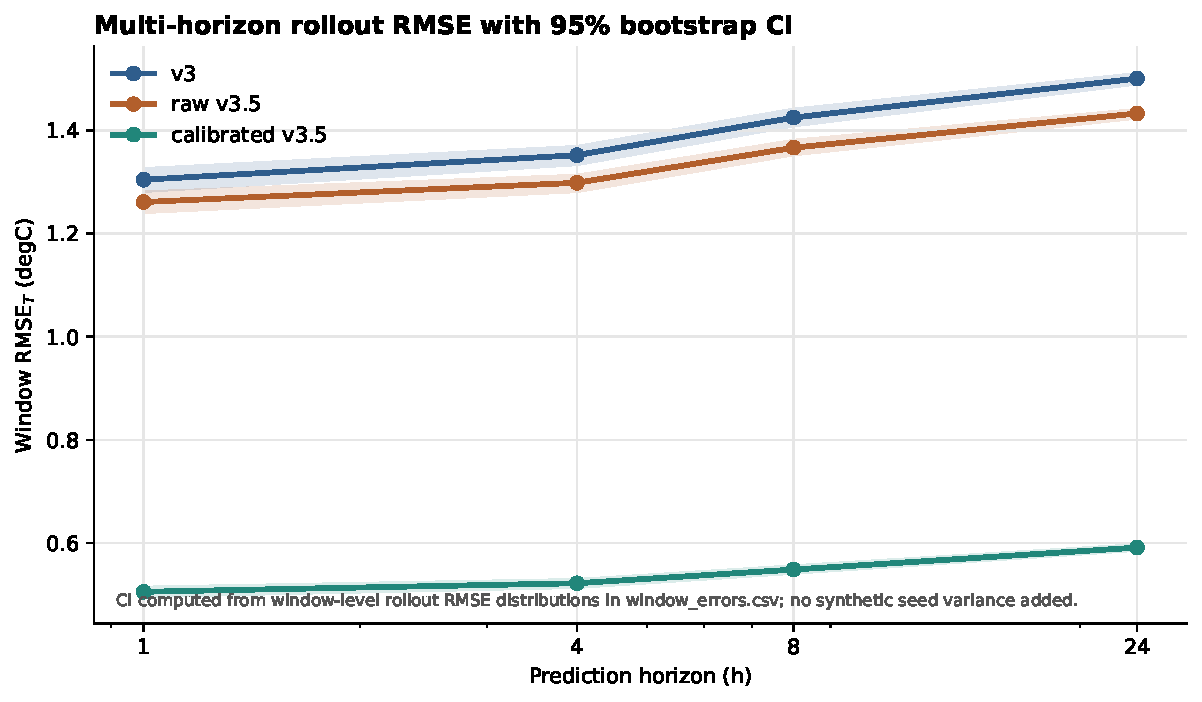
\includegraphics[width=0.95\linewidth]{block1_q1_polish_multi_horizon_ci.pdf}
  \caption{Multi-horizon rollout RMSE with 95\% bootstrap confidence intervals.
  Bands are computed from the real window-level rollout errors in
  \texttt{window\_errors.csv}; no synthetic seed variance is added.}
  \label{fig:multi-horizon}
\end{figure}

The calibrated v3.5 24 h rollout error is \(\SI{0.644}{\celsius}\), compared
with \(\SI{1.466}{\celsius}\) for raw v3.5 and \(\SI{1.557}{\celsius}\) for
the legacy v3 reference.

\subsection{Residual distribution and error CDF}

The signed residual is
\begin{equation}
  e_T = \widehat{T} - T_{\mathrm{BOPTEST}},
\end{equation}
and the engineering tolerance CDF is
\begin{equation}
  F_{\mathrm{abs}}(\epsilon)=\Pr(|e_T|\leq\epsilon).
  \label{eq:error-cdf}
\end{equation}

\begin{figure}[htbp]
  \centering
  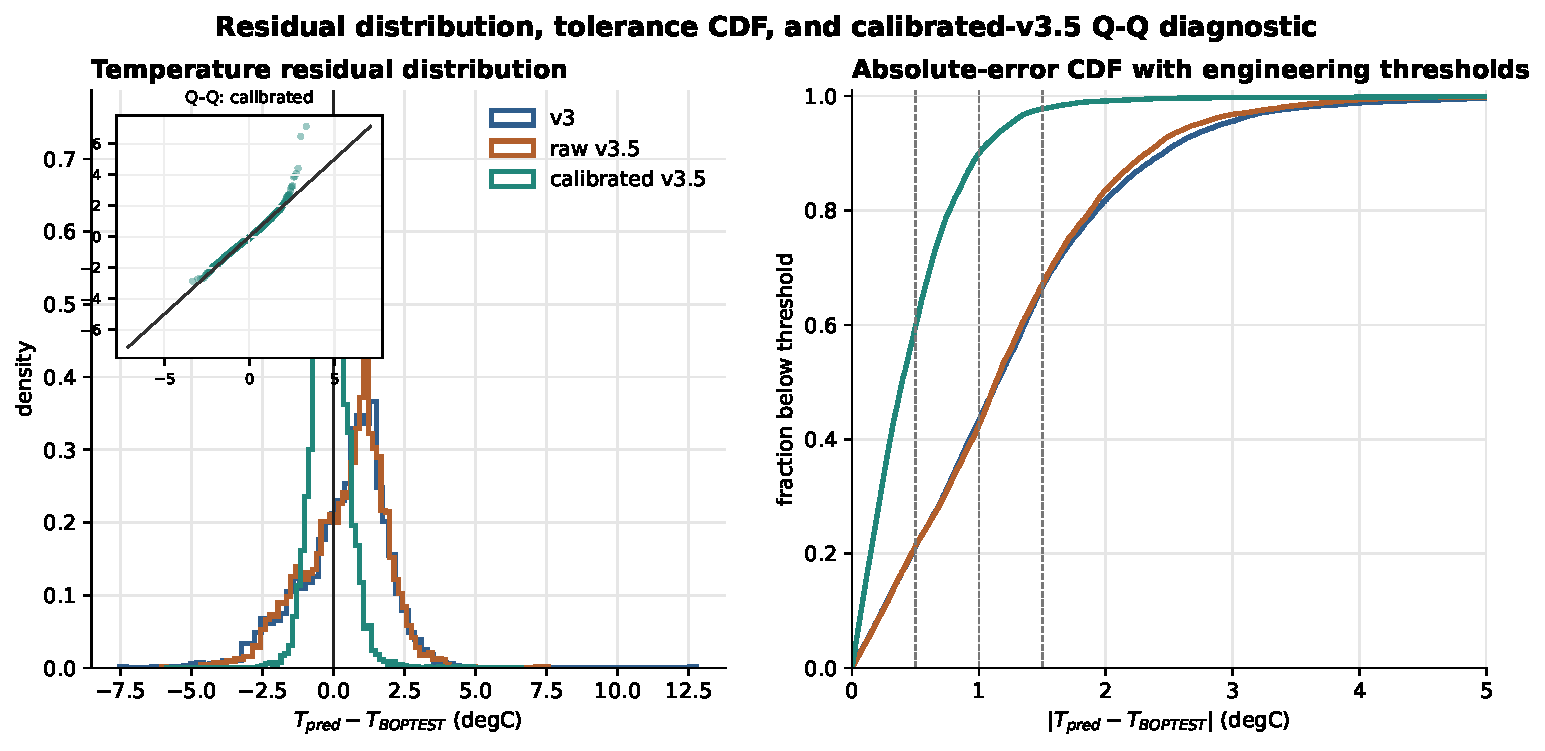
\includegraphics[width=0.95\linewidth]{block1_q1_polish_residual_distribution_qq_cdf.pdf}
  \caption{Residual distribution, absolute-error CDF, and calibrated-v3.5 Q-Q
  inset. The CDF reports engineering tolerance compliance, while the Q-Q inset
  checks whether calibrated residuals behave like approximately Gaussian
  residual noise rather than systematic drift.}
  \label{fig:residual-cdf}
\end{figure}

This diagnostic is more engineering-relevant than RMSE alone: it exposes bias,
spread, tail risk, and tolerance compliance.

\subsection{Replicative validity}

\begin{figure}[htbp]
  \centering
  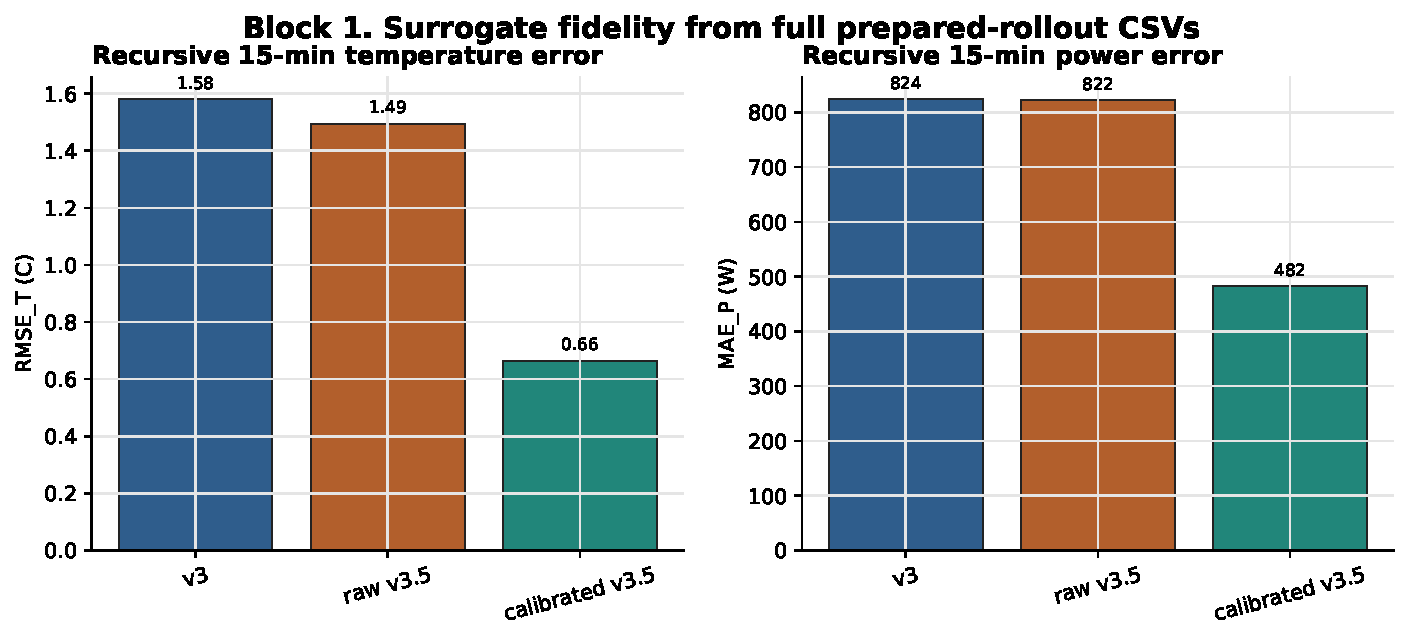
\includegraphics[width=0.90\linewidth]{block1_replicative_validity_bars.pdf}
  \caption{Per-episode rollout validity across held-out BOPTEST episodes.}
  \label{fig:replicative}
\end{figure}

\begin{figure}[htbp]
  \centering
  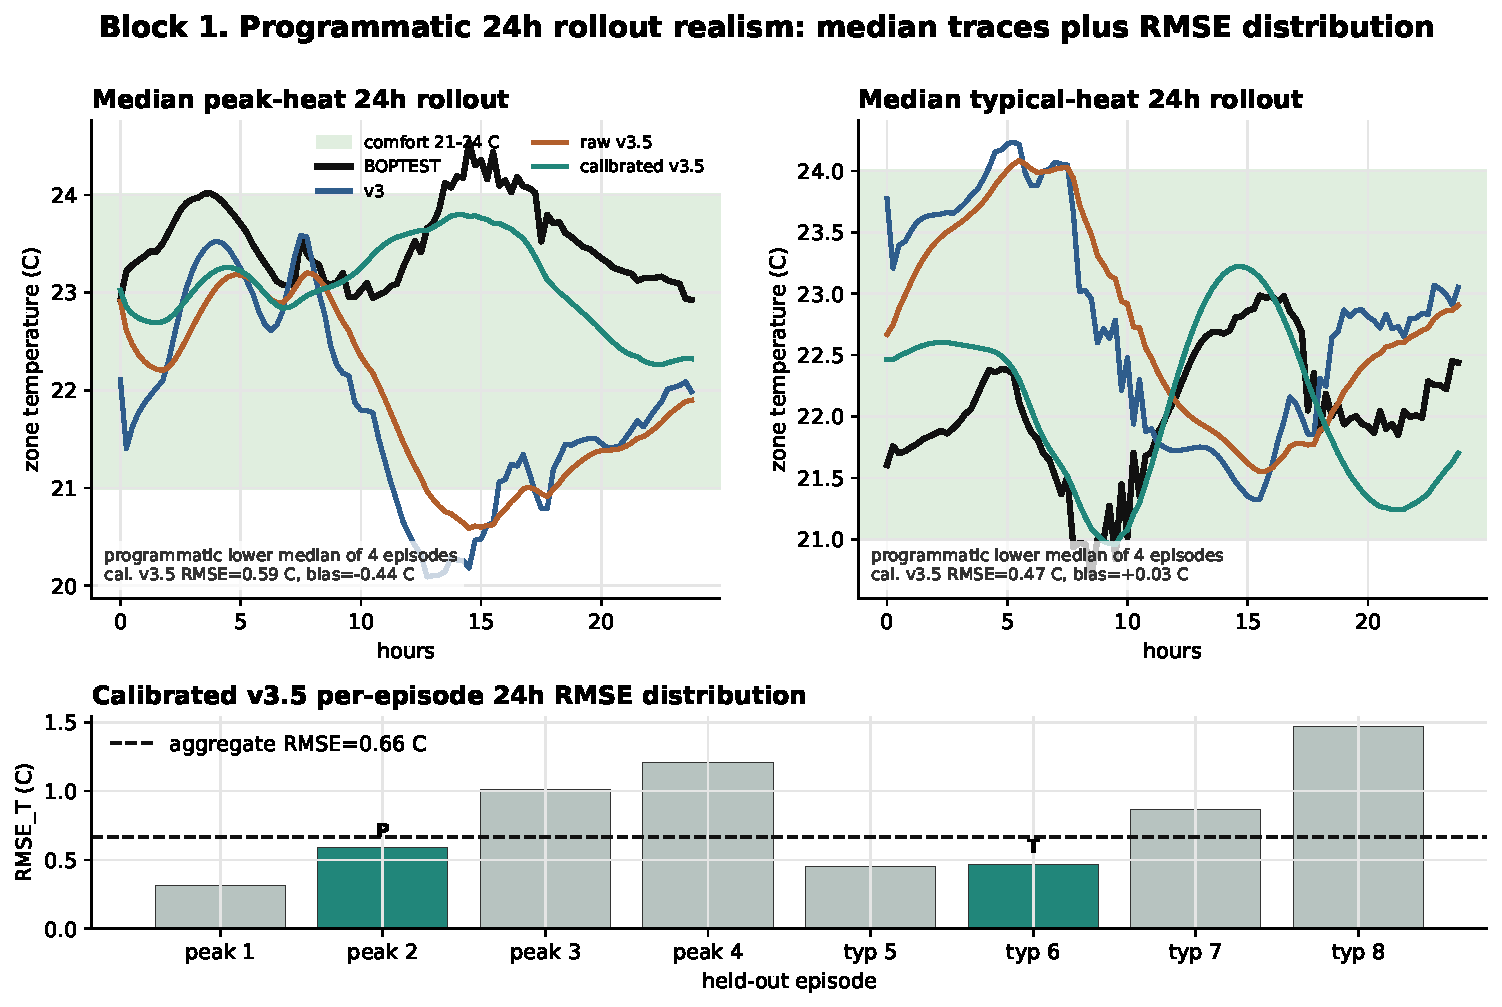
\includegraphics[width=0.95\linewidth]{block1_rollout_24h_temperature_trace.pdf}
  \caption{Representative 24 h rollout trace. The trace-level view complements
  the aggregate RMSE curves by showing time-local drift and recovery.}
  \label{fig:rollout-trace}
\end{figure}

\section{Matched-corpus control experiment}

A direct comparison between legacy v3 and v3.5 would be confounded by corpus
resolution. The legacy v3 reference was trained on hourly telemetry, whereas
v3.5 uses a 15-minute prepared corpus. The matched-corpus control experiment
therefore retrains v3 on the same 15-minute corpus used by v3.5.

\begin{table}[htbp]
\centering
\caption{Matched-corpus comparison for 24 h rollout RMSE.}
\label{tab:matched-corpus}
\begin{tabular}{p{0.24\linewidth}p{0.28\linewidth}p{0.16\linewidth}p{0.18\linewidth}}
\toprule
Variant & Corpus & Stage A/B/C & 24 h \(\RMSE_T\) \\
\midrule
v3 hourly & 51,200 hourly transitions & n/a & \(\SI{1.557}{\celsius}\) \\
v3 15-min matched & 10,744 15-min transitions & n/a & \(\SI{0.876}{\celsius}\) \\
raw v3.5 & 10,744 15-min transitions & off & \(\SI{1.466}{\celsius}\) \\
calibrated v3.5 & 10,744 15-min transitions & full & \(\SI{0.644}{\celsius}\) \\
\bottomrule
\end{tabular}
\end{table}

\begin{figure}[htbp]
  \centering
  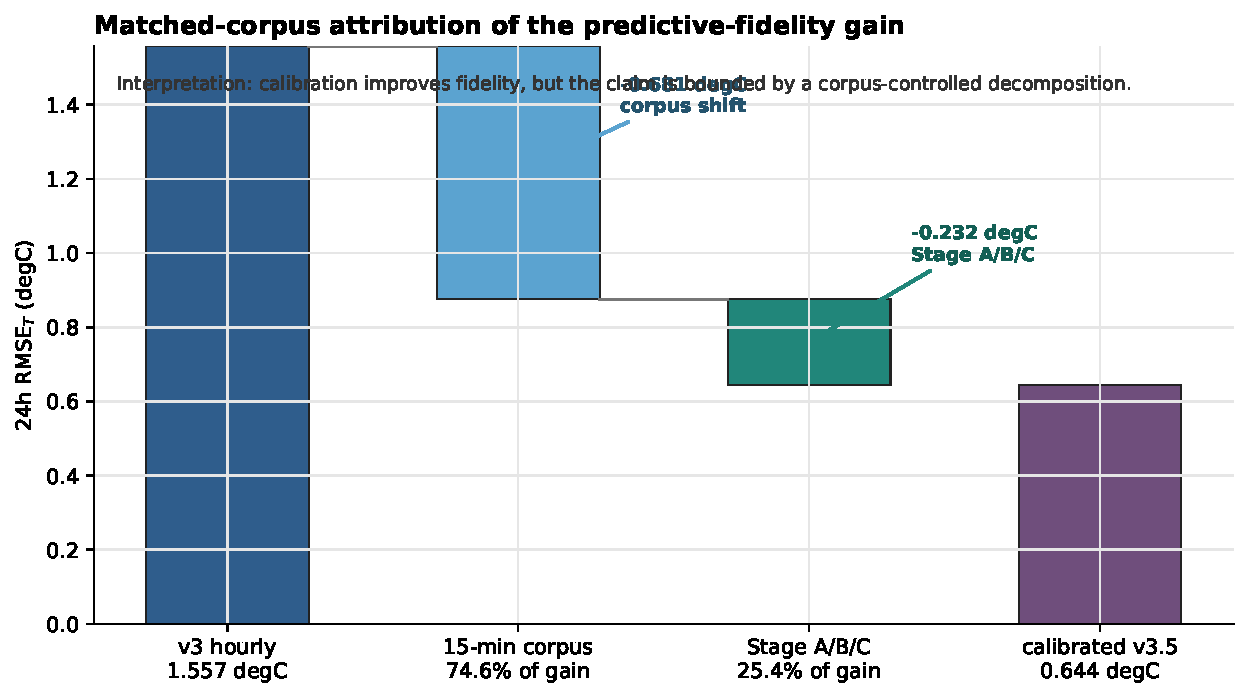
\includegraphics[width=0.90\linewidth]{block1_q1_polish_matched_waterfall.pdf}
  \caption{Matched-corpus waterfall decomposition. The accented arrows separate
  the \(15\)-min corpus contribution (\(-0.681\,^\circ\mathrm{C}\), 74.6\% of
  the gain) from the Stage A/B/C calibration contribution
  (\(-0.232\,^\circ\mathrm{C}\), 25.4\% of the gain).}
  \label{fig:matched-corpus}
\end{figure}

The decomposition is
\begin{align}
  \Delta_{\mathrm{total}} &= 1.557 - 0.644 = \SI{0.913}{\celsius},\\
  \Delta_{\mathrm{corpus}} &= 1.557 - 0.876 = \SI{0.681}{\celsius},\\
  \Delta_{\mathrm{cal}} &= 0.876 - 0.644 = \SI{0.232}{\celsius}.
\end{align}
Thus
\begin{equation}
  \frac{\Delta_{\mathrm{corpus}}}{\Delta_{\mathrm{total}}}=74.6\%,
  \qquad
  \frac{\Delta_{\mathrm{cal}}}{\Delta_{\mathrm{total}}}=25.4\%.
\end{equation}
The calibration claim is therefore real but bounded. The paper does not claim
that physics alone explains the full improvement; corpus resolution and
physical calibration jointly produce the final fidelity gain.

\section{Runtime benchmark}

For RL, surrogate fidelity is insufficient if the model is too slow for policy
optimization. The runtime benchmark compares the live BOPTEST RTE loop against
local surrogate stepping under the same 15-minute control protocol.

\begin{table}[htbp]
\centering
\caption{Backend simulation throughput.}
\label{tab:speed}
\begin{tabular}{lcc}
\toprule
Backend & Environment steps/s & Speed-up vs BOPTEST \\
\midrule
BOPTEST RTE HTTP loop & 21.0 & \(1.0\times\) \\
v3 surrogate & 4626.3 & \(220.2\times\) \\
v3.5 calibrated & 2399.5 & \(114.2\times\) \\
Hybrid v3+v3.5 & 1786.8 & \(85.0\times\) \\
\bottomrule
\end{tabular}
\end{table}

\begin{figure}[htbp]
  \centering
  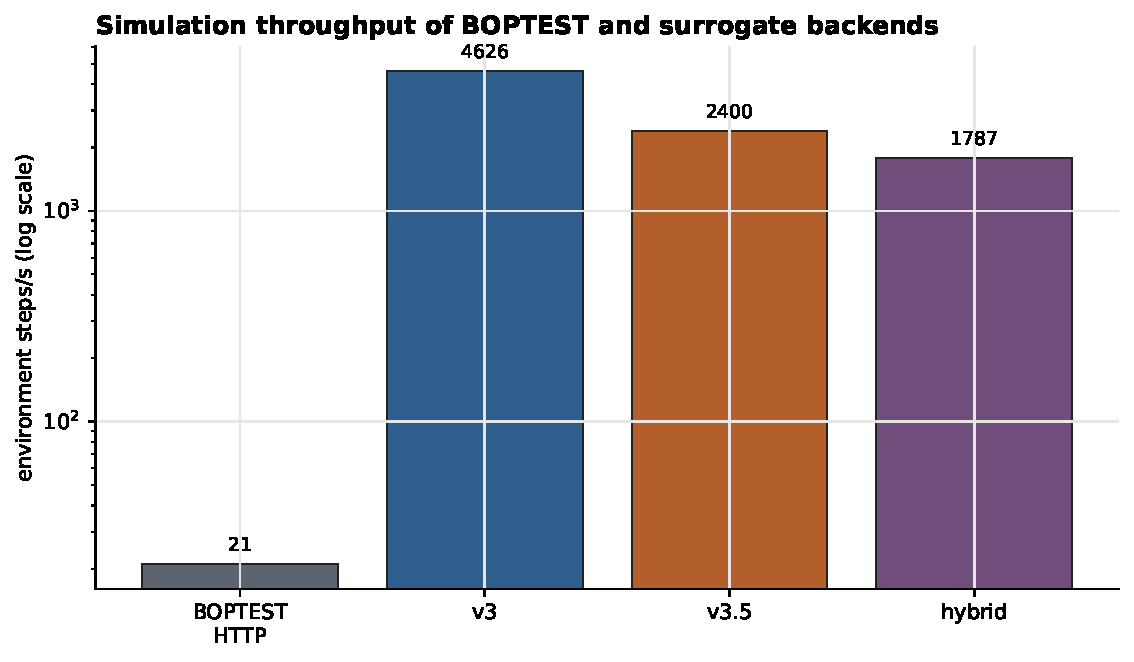
\includegraphics[width=0.85\linewidth]{block1_q1_fig09_backend_speed.pdf}
  \caption{Runtime benchmark of BOPTEST and surrogate backends.}
  \label{fig:speed}
\end{figure}

The hybrid backend is slower than v3 alone, but remains fast enough for PPO:
about \(85\times\) faster than the live BOPTEST HTTP-Docker validation loop.

\section{Hybrid backend: architecture and reward}

The direct-v3.5 negative result motivates the hybrid backend. The hybrid does
not replace v3 with v3.5. Instead, it separates their roles:
\begin{itemize}
  \item v3 generates rollout transitions for PPO;
  \item frozen v3.5 evaluates the same state-action pair;
  \item disagreement between v3 and v3.5 is penalized in the reward.
\end{itemize}

The hybrid reward is
\begin{equation}
  r_{\mathrm{hybrid}}
  =
  r_{\mathrm{comfort}}
  +
  r_{\mathrm{smooth}}
  +
  r_{\mathrm{energy}}
  -
  \lambda_T |T_{v3}-T_{v3.5}|
  -
  \lambda_P |P_{v3}-P_{v3.5}|.
  \label{eq:hybrid-reward}
\end{equation}

\begin{figure}[htbp]
  \centering
  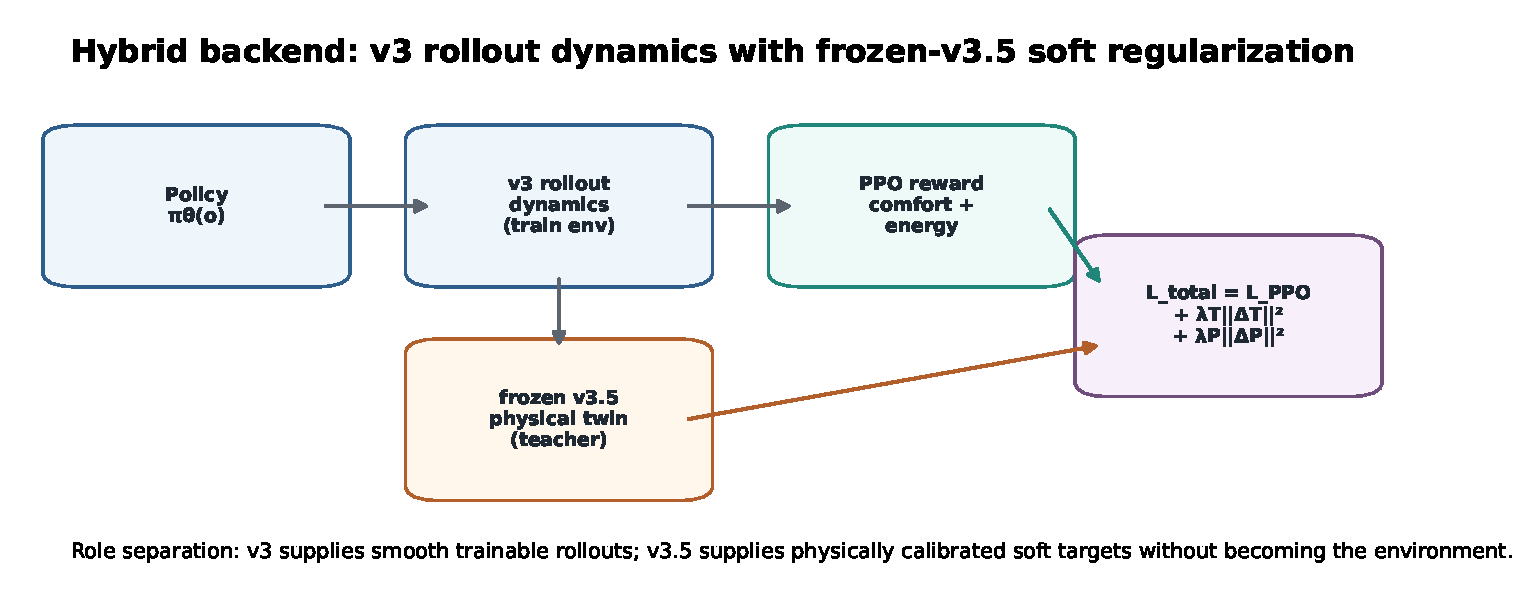
\includegraphics[width=0.95\linewidth]{block1_q1_fig14_hybrid_loss.pdf}
  \caption{Hybrid backend mechanism: v3 rollout dynamics with frozen-v3.5
  soft regularization.}
  \label{fig:hybrid-loss}
\end{figure}

The key engineering decision is that v3.5 contributes a physical consistency
cost but does not define the rollout transition. This is what prevents the
direct-v3.5 failure mode while retaining physical information.

\section{Fidelity-to-RL gap}

\begin{figure}[htbp]
  \centering
  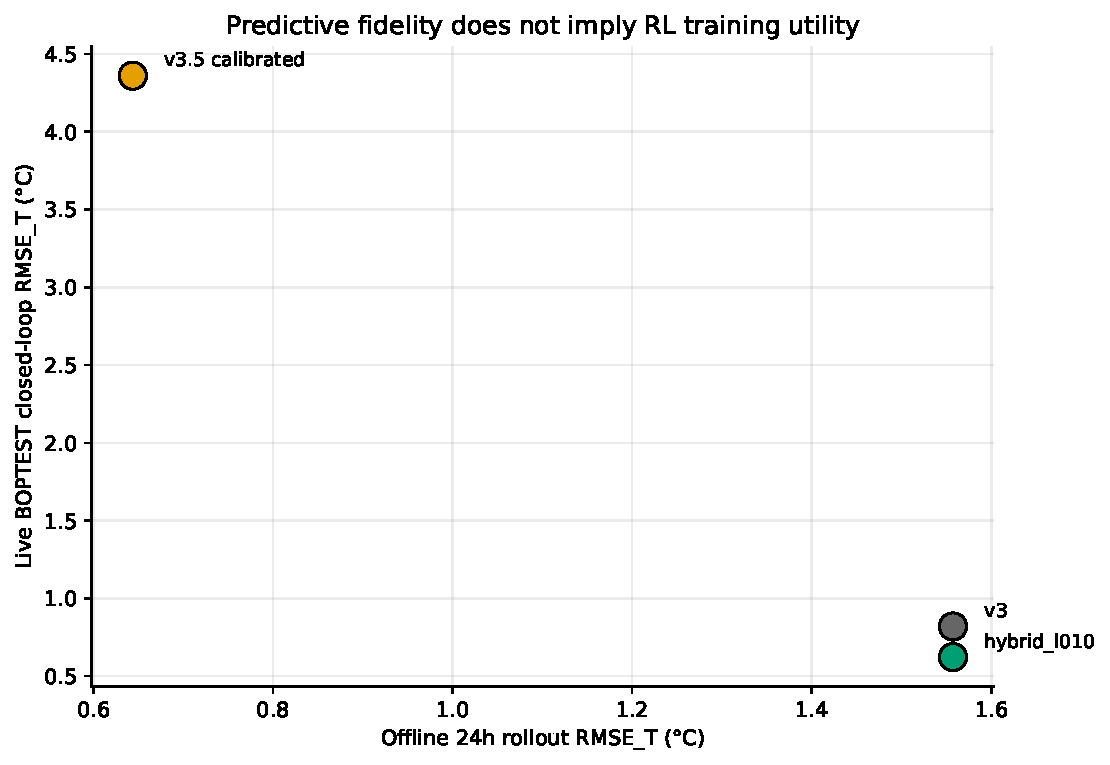
\includegraphics[width=0.82\linewidth]{final17_fig05_fidelity_vs_rl_utility.pdf}
  \caption{Predictive fidelity versus live control utility. Calibrated v3.5 is
  the strongest offline predictor but the weakest direct RL rollout backend.}
  \label{fig:fidelity-vs-control}
\end{figure}

\begin{figure}[htbp]
  \centering
  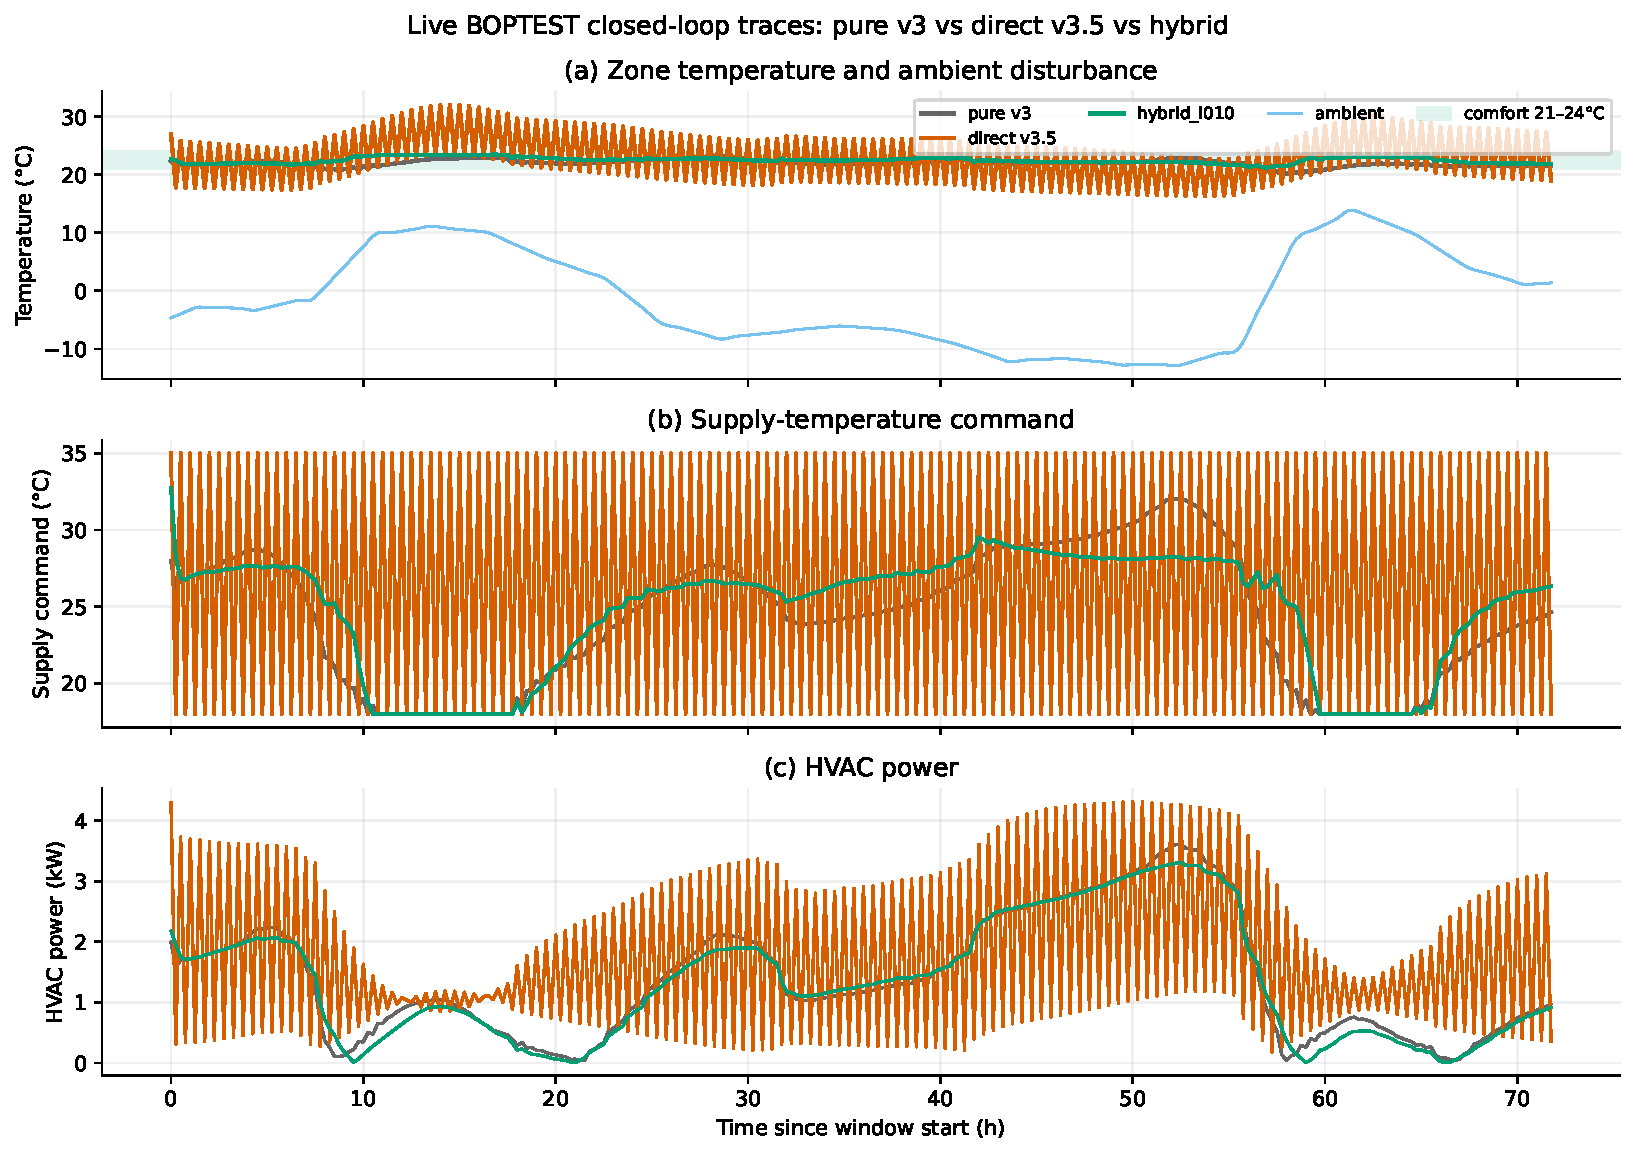
\includegraphics[width=0.95\linewidth]{final_eng_fig08_live_boptest_closed_loop_traces.pdf}
  \caption{Live BOPTEST closed-loop traces for pure v3, direct v3.5, and
  hybrid\_l010.}
  \label{fig:live-traces}
\end{figure}

The direct-v3.5 policy fails live BOPTEST despite v3.5 being the better
predictive model. It reaches approximately
\(\SI{4.32}{\celsius}\)--\(\SI{4.40}{\celsius}\) live temperature RMSE with
comfort violation around 77--82\%. In contrast, hybrid\_l010 reaches about
\(\SI{0.61}{\celsius}\)--\(\SI{0.63}{\celsius}\) live RMSE with low
single-digit violation.

This is the central negative result of Block 1:
\begin{quote}
  better predictive fidelity does not imply better RL training utility.
\end{quote}

\section{Transfer-gap diagnostics and action saturation}

The failure mechanism is visible in policy diagnostics.

\begin{figure}[htbp]
  \centering
  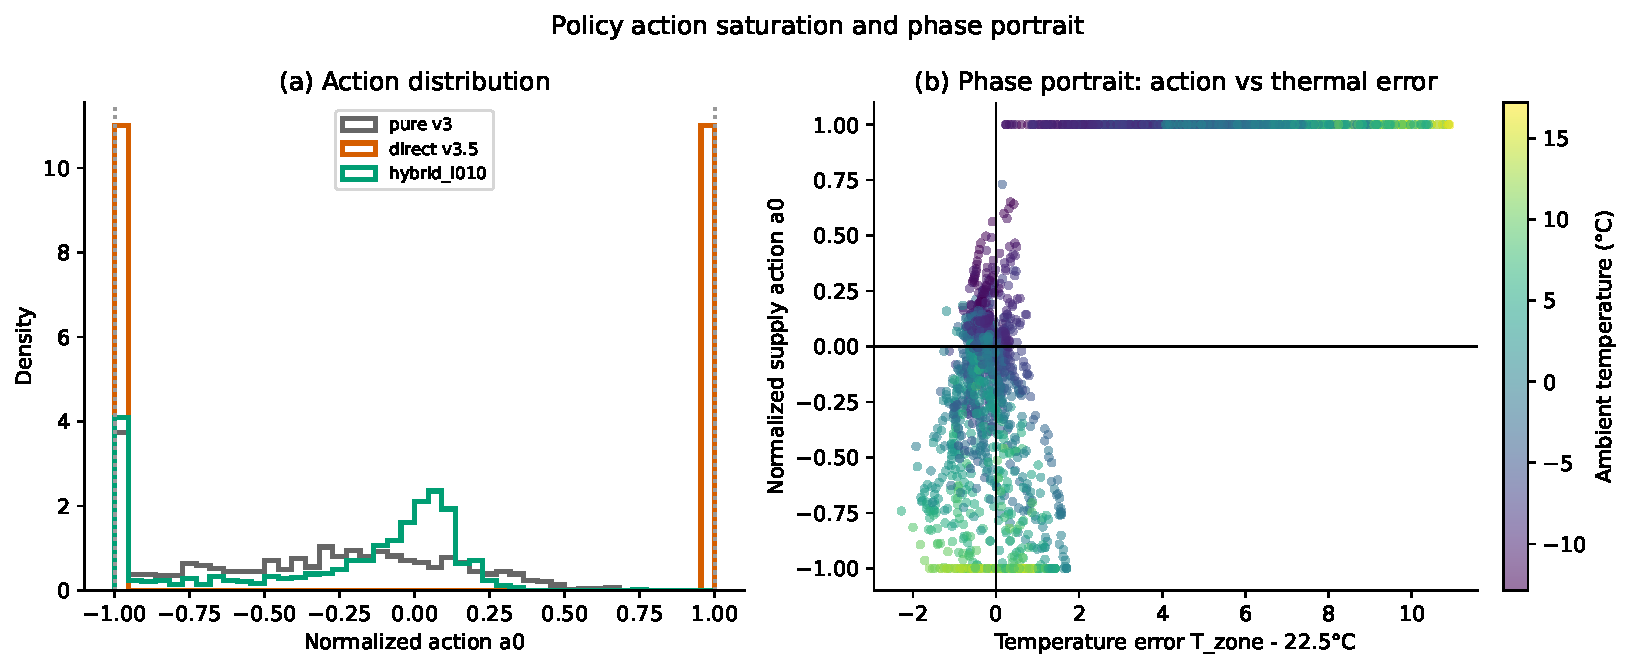
\includegraphics[width=0.95\linewidth]{final_eng_fig09_action_distribution_phase_portrait.pdf}
  \caption{Action distribution and phase portrait. Direct v3.5 PPO exhibits
  bang-bang action saturation and extreme action response relative to
  temperature error.}
  \label{fig:action-phase}
\end{figure}

\begin{figure}[htbp]
  \centering
  
\includegraphics[width=0.90\linewidth]{block1_q1_fig10_transfer_gap_diagnostics.pdf}
  \caption{Transfer-gap diagnostics across pure v3, direct v3.5, and
  hybrid\_l010.}
  \label{fig:transfer-gap}
\end{figure}

The transfer-gap diagnostic compares live BOPTEST behavior against surrogate
predictions. A useful backend should not only predict well offline; it should
also produce a policy whose behavior remains stable under live RTE deployment.
Direct v3.5 has a large action-gap norm around 2.0 and immediate divergence.
Hybrid\_l010 reduces the live/surrogate \(\ms\) gap to approximately 0.02 on
the targeted windows and delays or reduces divergence relative to direct v3.5.

\section{Block 1 conclusion}

Block 1 closes with a deliberately asymmetric conclusion.

\paragraph{Predictive digital twin.}
Calibrated v3.5 is supported. Stage A/B/C reduces 24 h rollout \(\RMSE_T\)
from \(\SI{1.466}{\celsius}\) to \(\SI{0.644}{\celsius}\), reduces power MAE
from \(\SI{810}{W}\) to \(\SI{482}{W}\), and identifies a physically plausible
\(\Czon=4.413\times10^5~\mathrm{J/K}\). The residual distribution, error CDF,
and Stage-B convergence diagnostics show that this is not a single-metric
artifact.

\paragraph{Direct RL rollout backend.}
Calibrated v3.5 is rejected as a direct RL environment. PPO trained directly on
v3.5 enters saturated action regimes and fails live BOPTEST validation despite
the model's stronger offline predictive fidelity.

\paragraph{Hybrid role separation.}
The constructive outcome is role separation. v3 remains the rollout backend
because it provides smooth and computationally cheap dynamics for PPO.
Calibrated v3.5 is retained as a frozen physical teacher through disagreement
regularization. This conclusion is the dependency passed to Block 2: controller
validation must test the hybrid role assignment, not merely compare surrogate
RMSE values.

\end{document}
